% THIS TEMPLATE IS A WORK IN PROGRESS

\documentclass[polish, a4paper]{article}
\usepackage[a4paper,left=3cm,right=3cm,top=3cm,bottom=1.5cm]{geometry}
\usepackage[T1]{fontenc}
\usepackage[polish]{babel}
\usepackage[utf8]{inputenc}
\usepackage{hyperref}
\usepackage{fancyhdr}
\usepackage{float}
\usepackage{graphicx}
\usepackage{titling}
\usepackage{wasysym}
\usepackage{caption}
\usepackage{pgfplots}
\usepackage{pgfplotstable}
\usepackage{filecontents}
\usepackage{csvsimple}
\usepackage{textcomp}
\usepackage{gensymb}
\usepackage{etoolbox}
\usepackage{enumitem}
\usepackage[style=iso]{datetime2}
%\usepackage{siunitx}
\graphicspath{ {./} }
\pagestyle{fancy}

\setlength{\droptitle}{-1in}

%\lhead{\includegraphics[width=0.2\textwidth]{nyush-logo.pdf}}

  \lhead{System zarządzający wynikami w kręglarstwie klasycznym}
\chead{}
\rhead{Inżynieria Oprogramowania}


%%%% PROJECT TITLE
\title{\vspace{3ex} System zarządzający wynikami w kręglarstwie klasycznym}

%%%% NAMES OF ALL THE STUDENTS INVOLVED (first-name last-name)
\author{Zespół nr 3}

\date{\vspace{-8ex}} %NO DATE


\begin{document}

\renewcommand{\labelenumii}{\arabic{enumi}.\arabic{enumii}}
\renewcommand{\labelenumiii}{\arabic{enumi}.\arabic{enumii}.\arabic{enumiii}}
\renewcommand{\labelenumiv}{\arabic{enumi}.\arabic{enumii}.\arabic{enumiii}.\arabic{enumiv}}

\maketitle
%\thispagestyle{titlepage}

\begin{table}[H]
\resizebox{\textwidth}{!}{%
\begin{tabular}{|c|c|c|c|}
\hline
\textbf{Wersja} & \textbf{Data utworzenia} & \textbf{Data ost. modyfikacji} & \textbf{Autorzy}                                                                         \\ \hline
1.3             & 2023-11-19               & 2024-01-25                     & \begin{tabular}[c]{@{}c@{}}Alan Grądecki 151126\\ Adam Jałocha 154020\\ Maciej Kaszkowiak 151856 \\ Mikołaj Gostkowski 151759\end{tabular} \\ \hline
\end{tabular}%
}
\end{table}

\tableofcontents

\newpage



\section{Informacje ogólne}

System zarządzajacy wynikami w kręglarstwie klasycznym przeznaczony jest do grupy zawodników i osób powiązanych z szeroko pojętym kręglarstwem klasycznym na terenie Polski. Celem systemu jest usprawnienie procesu przechowywania wyników, umożliwienie przetwarzania ich oraz ułatwienie analizy wyników poszczególnych zawodników i z poszczególnych zawodów. 

System powinien być możliwy do wykorzystania przez możliwie najszerszą grupę użytkowników, przez co jego interfejs powinien spełniać normy dostępności oraz być intuicyjny, również dla osób nieobytych z technologią. W celu poprawy jakości kręglarstwa klasycznego w Polsce, system powinien ułatwić analizę danych oraz wyciąganie wniosków z gry poszczególnych zawodników. Docelowo, każda zainteresowana osoba, powinna otrzymać dostęp do archiwum gier swoich (jako zawodnik), swoich podopiecznych (jako trener w klubie), czy na swojej kręgielni (jako klub sportowy). Ponadto, system ułatwi organizację turniejów sportowych, które dotychczas przechowują wyniki bez przyjęcia ustalonej konwencji przechowywania danych.

Odbiorcy docelowi naszego systemu składają się z 4 głównych segmentów:

\begin{description}
\item[Zawodnicy]{nie mają dostępu do swojej archiwalnej bazy wyników. Jedyny sposób na prowadzenie historii, to ręczne zbieranie fizycznych wydruków z automatów kręglarskich. System ułatwi im dostęp do swoich historycznych danych oraz ułatwi analizę gier i śledzenie postępów.}
\item[Trenerzy]{nie mają dostępu do bazy wyników swoich podopiecznych. Postęp swoich zawodników przeważnie mierzą w sposób empiryczny, opierając się na swojej ocenie, nie biorąc pod uwagę w pełni surowych danych z zawodów. System umożliwi im zwizualizowanie trendów wyników swoich zawodników na podstawie wykresów oraz ułatwi wyłanianie najlepszych zawodników na dane zawody.}
\item[Kluby sportowe]{nie posiadają pełnej historii gier swoich podopiecznych. Często również nie posiadają pełnej historii gier rozegranych na swoim obiekcie, ponieważ wyniki są zapisywane w sposób niezorganizowany oraz rozproszone na wielu kontach w Google Docs. System ułatwi im organizowanie turniejów, usprawnianie procesu wprowadzania wyników, a także zapewni pełną historię gier rozegranych na obiekcie.}
\item[Polski Związek Kręglarski]{wyłania zawodników do reprezentowania Polski na podstawie subiektywnych pomiarów trenerów, ponieważ nie istnieje obecnie system, który umożliwiłby ustalenie aktualnie najmocniejszych zawodników na podstawie danych z gier. System rozwiązałby ten problem, wspomagając PZK w podejmowaniu decyzji. Ponadto system uprościłby ustalanie rekordów Polski.}
\end{description}

Korzyści biznesowe systemu będą zauważalne w skali całej Polski. Przede wszystkim, ułatwiona analiza danych przyczyni się do zwiększenia poziomu poszczególnych zawodników, a co za tym idzie, całej dyscypliny oraz poziomu na scenie międzynarodowej. Organizowanie turniejów oraz trenowanie zawodników stanie się również prostszym procesem, co zwiększy możliwości poszczególnych klubów kręglarskich w zakresie maksymalnej liczby zawodników oraz zawodów. Ponadto system ułatwia życie w niemierzalny sposób, eliminując ręczne bariery wymagane do zarządzania wynikami. 

\section{Diagram kontekstu}

\begin{figure}[H]
  \centering
  \includegraphics[width=\textwidth]{diagram.png}
  \caption{Diagram kontekstu}
\end{figure}

\section{Aktorzy}

W systemie wyróżniamy następujących aktorów:

\begin{description}
\item[Zawodnik]{ jest użytkownikiem w systemie. Ma możliwość wprowadzania danych ze swoich treningów. Posiada dostęp do swoich historycznych danych oraz może je przeanalizować za pomocą wykresów otrzymanych ze systemu.}
\item[Trener]{ jest użytkownikiem w systemie. Ma możliwość wprowadzania planów treningowych dla swoich zawodników. Może podejrzeć listę nadchodzących zawodów oraz wyniki i dane swoich zawodników. Trener przynależy do klubu.}
\item[Klub]{ jest użytkownikiem w systemie. Ma możliwość zarządzania trenerami oraz zawodnikami. Klub może organizować zawody oraz jest odpowiedzialny za wprowadzanie w ich obrębie wyników. Klub posiada dostęp do pełnej historii gier na obiekcie.}
\item[Administrator]{ jest użytkownikiem w systemie. Ma możliwość korekty błędnie wprowadzonych danych przez kluby kręglarskie. Zarządza klubami kręglarskimi. Ma dostęp do pełnej historii gier oraz do nieograniczonej analizy w zakresie wszystkich dostępnych wyników.}
\item[Automat]{ jest potencjalnym miejscem integracji z urządzeniem elektronicznym zapisującym wyniki na kręgielni. Wyniki zawodników mogą zostać automatycznie zapisane do zawodów. Automatycznie może również wyświetlać się imie i nazwisko danego zawodnika w trakcie jego gry.}
\end{description}

Wszyscy użytkownicy mają dostęp do zawodów oraz do wyników poszczególnych zawodników w ramach zawodów, również Ci niezalogowani.

% aktorzy = role uzytkownikow w systemie

\section{Wymagania funkcjonalne}
\subsection{Diagram przypadków użycia}

\begin{figure}[H]
  \centering
  \includegraphics[width=\textwidth]{diagram_uml2.png}
  \caption{Diagram przypadków użycia}
\end{figure}



\subsection{Przypadki użycia}


% start
\subsubsection{Dodawanie wyników zawodnika}
\noindent
\textbf{Atrybuty:}
\begin{description}[labelindent=0.5cm]
    \item[Główny aktor:]{Klub}
    \item[Priorytet:]{Wysoki}
    \item[Źródło:]{Mikołaj Gostkowski}
\end{description}

\noindent
\textbf{Główny scenariusz:}
\begin{enumerate}
    \item Klub wyszukuje danego zawodnika na liście
    \item Klub wprowadza uzyskane przez danego zawodnika punkty
    \item Klub zatwierdza zmiany
    \item Wyniki zawodnika są widoczne w systemie
\end{enumerate}


\subsubsection{Wyświetlanie historycznych wyników zawodnika}
\noindent
\textbf{Atrybuty:}
\begin{description}[labelindent=0.5cm]
    \item[Główny aktor:]{Zawodnik lub Trener lub Klub lub Administrator}
    \item[Priorytet:]{Wysoki}
    \item[Źródło:]{Maciej Kaszkowiak}
\end{description}

\noindent
\textbf{Główny scenariusz:}
\begin{enumerate}
    \item Zawodnik, trener, klub lub administrator dokonuje wyboru danego zawodnika z listy
    \item Zawodnik, trener, klub lub administrator dokonuje wyboru okresu czasu
    \item Historyczne wyniki zawodnika z wybranego okresu zostają wyświetlone
\end{enumerate}
\noindent
\textbf{Rozszerzenia:}
\begin{itemize}
    \item[1.A] Zawodnik może wyświetlić tylko własne historyczne wyniki
\end{itemize}


\subsubsection{Korekta wyników zawodników}
\noindent
\textbf{Atrybuty:}
\begin{description}[labelindent=0.5cm]
    \item[Główny aktor:]{Klub lub Administrator}
    \item[Priorytet:]{Średni}
    \item[Źródło:]{Alan Grądecki}
\end{description}

\noindent
\textbf{Główny scenariusz:}
\begin{enumerate}
    \item Klub lub administrator wybiera zawodnika z listy
    \item Klub lub administrator wybiera dane zawody
    \item Klub lub administrator dokonuje korekty wyniku
    \item Klub lub administrator zatwierdza zmiany
    \item Zaktualizowane wyniki zawodnika są widoczne na liście danych zawodów
\end{enumerate}

\subsubsection{Generowanie wykresów sprawności zawodnika}
\noindent
\textbf{Atrybuty:}
\begin{description}[labelindent=0.5cm]
    \item[Główny aktor:]{Zawodnik lub Trener lub Klub}
    \item[Priorytet:]{Wysoki}
    \item[Źródło:]{Adam Jałocha}
\end{description}

\noindent
\textbf{Główny scenariusz:}
\begin{enumerate}
    \item Zawodnik, trener lub klub dokonuje wyboru zawodnika z listy
    \item Zawodnik, trener lub klub generuje wykresy sprawności danego zawodnika
    \item Wygenerowane wykresy są widoczne i można je wyeksportować z systemu
\end{enumerate}
\noindent
\textbf{Rozszerzenia:}
\begin{itemize}
    \item[1.A] Zawodnik może wybrać tylko siebie
    \item[2.A] Zawodnik może wygenerować tylko własne wykresy sprawności
\end{itemize}
% end

\subsubsection{Tworzenie zawodów kręglarskich}
\noindent
\textbf{Atrybuty:}
\begin{description}[labelindent=0.5cm]
    \item[Główny aktor:]{Klub}
    \item[Priorytet:]{Wysoki}
    \item[Źródło:]{Adam Jałocha}
\end{description}

\noindent
\textbf{Główny scenariusz:}
\begin{enumerate}
    \item Klub podaje szczegóły nowych zawodów.
    \item Klub zatwierdza formularz.
    \item Zawody zostają utworzone.
    \item Zawody są widoczne na ogólnodostępnej liście wszystkich zawodów.
\end{enumerate}
\noindent
\textbf{Rozszerzenia:}
\begin{itemize}
    \item[3.A] Klub po zatwierdzeniu błędnych danych zostaje przekierowany do punktu 1. wraz z odpowiednią informacją o popełnionych błędach, a zawody nie zostają utworzone.
\end{itemize}


\subsubsection{Synchronizacja wyników zawodnika}
\noindent
\textbf{Atrybuty:}
\begin{description}[labelindent=0.5cm]
    \item[Główny aktor:]{Automat}
    \item[Priorytet:]{Średni}
    \item[Źródło:]{Alan Grądecki}
\end{description}

\noindent
\textbf{Główny scenariusz:}
\begin{enumerate}
    \item Automat pobiera informacje o zawodniku znajdującego się na przypisanym torze, aby móc je wyświetlić.
    \item Automat śledzi grę użytkownika, notując wynik na przekroju wszystkich 4 torów.
    \item Automat po zakończonej grze zapisuje wynik zawodnika w systemie.
\end{enumerate}
\noindent
\textbf{Rozszerzenia:}
\begin{itemize}
    \item[3.A] Funkcjonalność jest opcjonalna, może zostać wyłączona w celu zapewnienia pełnej poprawności wyników.
\end{itemize}

\subsubsection{Dodawanie klubów}
\noindent
\textbf{Atrybuty:}
\begin{description}[labelindent=0.5cm]
    \item[Główny aktor:]{Administrator}
    \item[Priorytet:]{Średni}
    \item[Źródło:]{Adam Jałocha}
\end{description}

\noindent
\textbf{Główny scenariusz:}
\begin{enumerate}
    \item Administrator podaje dane nowego klubu.
    \item Administrator zatwierdza formularz.
    \item Klub zostaje utworzony.
    \item Klub otrzymuje dane dostępowe do systemu.
\end{enumerate}
\noindent
\textbf{Rozszerzenia:}
\begin{itemize}
    \item[3.A] Administrator po zatwierdzeniu błędnych danych zostaje przekierowany do punktu 1. wraz z odpowiednią informacją o popełnionych błędach, a klub nie zostaje utworzony.
\end{itemize}

\subsubsection{Dodawanie trenerów}
\noindent
\textbf{Atrybuty:}
\begin{description}[labelindent=0.5cm]
    \item[Główny aktor:]{Klub}
    \item[Priorytet:]{Wysoki}
    \item[Źródło:]{Maciej Kaszkowiak}
\end{description}

\noindent
\textbf{Główny scenariusz:}
\begin{enumerate}
    \item Klub podaje dane nowego trenera ze swojego klubu.
    \item Klub zatwierdza formularz.
    \item Trener zostaje utworzony.
    \item Trener otrzymuje dane dostępowe do systemu.
\end{enumerate}
\noindent
\textbf{Rozszerzenia:}
\begin{itemize}
    \item[3.A] Klub po zatwierdzeniu błędnych danych zostaje przekierowany na krok 1. wraz z odpowiednią informacją o popełnionych błędach, a trener nie zostaje utworzony.
\end{itemize}


\subsubsection{Dodawanie zawodników}
\noindent
\textbf{Atrybuty:}
\begin{description}[labelindent=0.5cm]
    \item[Główny aktor:]{Klub}
    \item[Priorytet:]{Wysoki}
    \item[Źródło:]{Mikołaj Gostkowski}
\end{description}

\noindent
\textbf{Główny scenariusz:}
\begin{enumerate}
    \item Klub podaje dane nowego zawodnika ze swojego klubu.
    \item Klub zatwierdza formularz.
    \item Zawodnik zostaje utworzony.
    \item Zawodnik otrzymuje dane dostępowe do systemu.
\end{enumerate}
\noindent
\textbf{Rozszerzenia:}
\begin{itemize}
    \item[3.A] Klub po zatwierdzeniu błędnych danych zostaje przekierowany na krok 1. wraz z odpowiednią informacją o popełnionych błędach, a zawodnik nie zostaje utworzony.
\end{itemize}



\subsubsection{Wyświetlanie historycznych rekordów}
\noindent
\textbf{Atrybuty:}
\begin{description}[labelindent=0.5cm]
    \item[Główny aktor:]{Administrator / Klub}
    \item[Priorytet:]{Niski}
    \item[Źródło:]{Maciej Kaszkowiak}
\end{description}

\noindent
\textbf{Główny scenariusz:}
\begin{enumerate}
    \item Członek PZK wchodzi w kręgielnię przypisaną do danego klubu. 
    \item Członek PZK widzi najlepsze wyniki osiągnięte na kręgielni.
    \item Najlepsze wyniki podlegają sortowaniu i filtrowaniu po wyniku, dacie i nazwie zawodnika. 
\end{enumerate}
\noindent
\textbf{Rozszerzenia:}
\begin{itemize}
    \item[1.A] Administrator może wejść w rekordy ze wszystkich obiektów.
\end{itemize}


\subsubsection{Wprowadzanie planów treningowych}
\noindent
\textbf{Atrybuty:}
\begin{description}[labelindent=0.5cm]
    \item[Główny aktor:]{Trener}
    \item[Priorytet:]{Niski}
    \item[Źródło:]{Mikołaj Gostkowski}
\end{description}

\noindent
\textbf{Główny scenariusz:}
\begin{enumerate}
    \item Trener wybiera datę treningu i zawodnika, dla którego zostanie przypisany plan.
    \item Trener wprowadza kolejne elementy treningu.
    \item Trener zatwierdza trening.
\end{enumerate}

\subsubsection{Realizowanie planów treningowych}
\noindent
\textbf{Atrybuty:}
\begin{description}[labelindent=0.5cm]
    \item[Główny aktor:]{Zawodnik / Trener}
    \item[Priorytet:]{Niski}
    \item[Źródło:]{Alan Grądecki}
\end{description}

\noindent
\textbf{Główny scenariusz:}
\begin{enumerate}
    \item Zawodnik wchodzi w listę planów treningowych.
    \item Zawodnik odczytuje szczegóły planu.
    \item Zawodnik dodaje wyniki treningowe.
    \item Zawodnik oznacza plan jako wykonany.
\end{enumerate}


\section{Wymagania pozafunkcjonalne}

\subsection{Użyteczność}
\begin{itemize}

\item System łatwy w obsłudze zarówno dla zawodników i jednostek zarządzających.\\ \emph{autor: Adam Jałocha}

\item Maksymalny czas szkolenia nie powinien przekroczyć godziny. \\ \emph{autor: Alan Grądecki}
  
\item Liczba kontaktów ze wsparciem klienta powinna być średnio bliska zeru, poza szczególnymi przypadkami i sytuacjami wyjątkowymi.\\ \emph{autor: Maciej Kaszkowiak}
  
\item Sytuacje w których konieczne jest skorzystanie z systemu pomocy powinno dotyczyć tylko osób niezaznajomionych z podstawowymi narzędziami internetowymi i osób niepełnosprawnych. Liczba takich sytuacji nie powinna przekraczać 5 na kwartał.\\ \emph{autor: Mikołaj Gostkowski}

\end{itemize}

\subsection{Niezawodność}
\begin{itemize}

\item Średnia liczba godzin pracy bez awarii nie powinna przekraczać tygodnia w ciągu roku. \\ \emph{autor: Maciej Kaszkowiak}
  
\item Prace konserwacyjne nie powinny przekroczyć 3 godzin w miesiącu i prace nad systemem 
powinny odbywać się w godzinach nocnych, w których system nie jest używany przez użytkowników. \\ \emph{autor: Alan Grądecki}
  
\item W przypadku awarii maksymalny czas przywrócenia systemu do sprawności nie powinien przekroczyć godziny i powinien zostać wyświetlony odpowiedni komunikat dla użytkownika z planowanymi pracami.\\ \emph{autor: Mikołaj Gostkowski}

\item Dane w systemie powinny być wprowadzane w sposób autoryzowany i ścisły, aby nie dochodziło do zachwiania spójności danych.  \\ \emph{autor: Adam Jałocha}

\end{itemize}

\subsection{Wydajność}

\begin{itemize}

\item System powinien wspierać przechowywanie danych dla co najmniej dziesięciokrotności liczebności wszystkich zawodników zapisanych w Polskim Związku Kręglarskim pod kątem zarejestrowanych kont.\\ \emph{autor: Adam Jałocha}

\item System powinien umożliwiać jednoczesny odczyt danych dla zawodów dla co najmniej jednokrotności wszystkich zawodników zapisanych w Polskim Związku Kręglarskim.\\ \emph{autor: Mikołaj Gostkowski}

\item P90 latency powinno wynosić do 200 ms, P95 latency do 300 ms, a P99 ms latency do 500 ms. \\ \emph{autor: Maciej Kaszkowiak}

\item System powinien wspierać jednoczesny zapis wyników z treningów dla 1/10 bazy zawodników. \\ \emph{autor: Alan Grądecki}

\end{itemize}



\subsection{Bezpieczeństwo}

\begin{itemize}

\item Wszystkie dane przechowywane w systemie, zwłaszcza dane osobowe zawodników, powinny być szyfrowane, aby zapewnić poufność informacji.\\ \emph{autor: Mikołaj Gostkowski}

\item System powinien wykorzystywać silny mechanizm szyfrowania - co najmniej Argon2 lub SHA512.\\ \emph{autor: Maciej Kaszkowiak}

\item Wdrożenie mechanizmów autoryzacji i uwierzytelniania, aby zapewnić dostęp do danych tylko uprawnionym użytkownikom.\\ \emph{autor: Alan Grądecki}

\item System powinien rejestrować wszelkie próby dostępu, modyfikacji danych lub innych aktywności, aby umożliwić śledzenie i reakcję na potencjalne zagrożenia.\\ \emph{autor: Adam Jałocha}

\item Zapewnienie zgodności z obowiązującymi przepisami o ochronie danych osobowych, takimi jak RODO, aby chronić prywatność użytkowników systemu.\\ \emph{autor: Maciej Kaszkowiak}

\end{itemize}


\section{Model systemu}
\subsection{Diagram klas}

\begin{figure}[H]
  \centering
  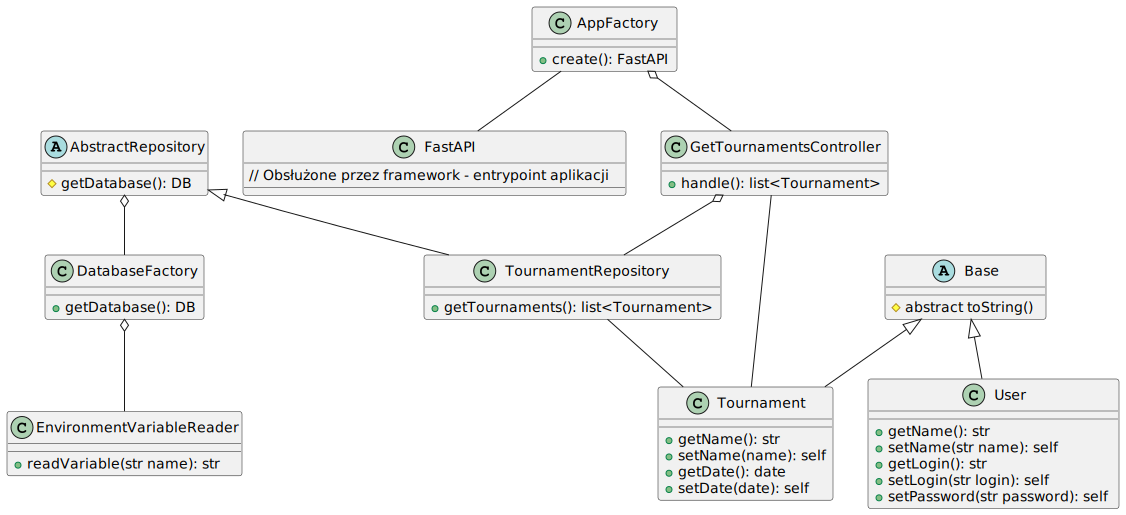
\includegraphics[width=\textwidth]{uml klasy.png}
  \caption{Diagram klas, autor: Maciej Kaszkowiak}
\end{figure}

\subsection{Diagram stanów}
\begin{figure}[H]
  \centering
  \includegraphics[width=\textwidth]{stan_turniej.png}
  \caption{Diagram stanów dla Tournament, autor: Adam Jałocha}
\end{figure}

\begin{figure}[H]
  \centering
  \includegraphics[width=\textwidth]{stan_user.png}
  \caption{Diagram stanów dla User, autor: Mikołaj Gostkowski}
\end{figure}

\subsection{Diagram sekwencji}

\begin{figure}[H]
  \centering
  \includegraphics[width=\textwidth]{sekw_dodawanie_wyn_zaw.png}
  \caption{Dodawanie wyników zawodnika, autor: Maciej Kaszkowiak}
\end{figure}

\begin{figure}[H]
  \centering
  \includegraphics[width=\textwidth]{sekw_korekta_wynikow_zaw.png}
  \caption{Korekta wyników zawodnika, autor: Mikołaj Gostkowski}
\end{figure}

\begin{figure}[H]
  \centering
  \includegraphics[width=\textwidth]{sekw_tworzenie_zawodow_kreg.png}
  \caption{Tworzenie zawodów kręglarskich, autor: Alan Grądecki}
\end{figure}

\begin{figure}[H]
  \centering
  \includegraphics[width=\textwidth]{sekw_wyswietlanie_historycznych_wynikow.png}
  \caption{Wyświetlenie historycznych wyników zawodnika, autor: Adam Jałocha}
\end{figure}

\subsection{Diagram wdrożenia}
\begin{figure}[H]
  \centering
  \includegraphics[width=\textwidth]{diagram_wdrozenia.png}
    \caption{Diagram wdrożenia, autor: Alan Grądecki}
\end{figure}
\end{document}